% Options for packages loaded elsewhere
\PassOptionsToPackage{unicode}{hyperref}
\PassOptionsToPackage{hyphens}{url}
\PassOptionsToPackage{dvipsnames,svgnames,x11names}{xcolor}
%
\documentclass[
  letterpaper,
  DIV=11,
  numbers=noendperiod]{scrartcl}

\usepackage{amsmath,amssymb}
\usepackage{iftex}
\ifPDFTeX
  \usepackage[T1]{fontenc}
  \usepackage[utf8]{inputenc}
  \usepackage{textcomp} % provide euro and other symbols
\else % if luatex or xetex
  \usepackage{unicode-math}
  \defaultfontfeatures{Scale=MatchLowercase}
  \defaultfontfeatures[\rmfamily]{Ligatures=TeX,Scale=1}
\fi
\usepackage{lmodern}
\ifPDFTeX\else  
    % xetex/luatex font selection
\fi
% Use upquote if available, for straight quotes in verbatim environments
\IfFileExists{upquote.sty}{\usepackage{upquote}}{}
\IfFileExists{microtype.sty}{% use microtype if available
  \usepackage[]{microtype}
  \UseMicrotypeSet[protrusion]{basicmath} % disable protrusion for tt fonts
}{}
\makeatletter
\@ifundefined{KOMAClassName}{% if non-KOMA class
  \IfFileExists{parskip.sty}{%
    \usepackage{parskip}
  }{% else
    \setlength{\parindent}{0pt}
    \setlength{\parskip}{6pt plus 2pt minus 1pt}}
}{% if KOMA class
  \KOMAoptions{parskip=half}}
\makeatother
\usepackage{xcolor}
\setlength{\emergencystretch}{3em} % prevent overfull lines
\setcounter{secnumdepth}{-\maxdimen} % remove section numbering
% Make \paragraph and \subparagraph free-standing
\ifx\paragraph\undefined\else
  \let\oldparagraph\paragraph
  \renewcommand{\paragraph}[1]{\oldparagraph{#1}\mbox{}}
\fi
\ifx\subparagraph\undefined\else
  \let\oldsubparagraph\subparagraph
  \renewcommand{\subparagraph}[1]{\oldsubparagraph{#1}\mbox{}}
\fi


\providecommand{\tightlist}{%
  \setlength{\itemsep}{0pt}\setlength{\parskip}{0pt}}\usepackage{longtable,booktabs,array}
\usepackage{calc} % for calculating minipage widths
% Correct order of tables after \paragraph or \subparagraph
\usepackage{etoolbox}
\makeatletter
\patchcmd\longtable{\par}{\if@noskipsec\mbox{}\fi\par}{}{}
\makeatother
% Allow footnotes in longtable head/foot
\IfFileExists{footnotehyper.sty}{\usepackage{footnotehyper}}{\usepackage{footnote}}
\makesavenoteenv{longtable}
\usepackage{graphicx}
\makeatletter
\def\maxwidth{\ifdim\Gin@nat@width>\linewidth\linewidth\else\Gin@nat@width\fi}
\def\maxheight{\ifdim\Gin@nat@height>\textheight\textheight\else\Gin@nat@height\fi}
\makeatother
% Scale images if necessary, so that they will not overflow the page
% margins by default, and it is still possible to overwrite the defaults
% using explicit options in \includegraphics[width, height, ...]{}
\setkeys{Gin}{width=\maxwidth,height=\maxheight,keepaspectratio}
% Set default figure placement to htbp
\makeatletter
\def\fps@figure{htbp}
\makeatother

\KOMAoption{captions}{tableheading}
\makeatletter
\@ifpackageloaded{caption}{}{\usepackage{caption}}
\AtBeginDocument{%
\ifdefined\contentsname
  \renewcommand*\contentsname{Table of contents}
\else
  \newcommand\contentsname{Table of contents}
\fi
\ifdefined\listfigurename
  \renewcommand*\listfigurename{List of Figures}
\else
  \newcommand\listfigurename{List of Figures}
\fi
\ifdefined\listtablename
  \renewcommand*\listtablename{List of Tables}
\else
  \newcommand\listtablename{List of Tables}
\fi
\ifdefined\figurename
  \renewcommand*\figurename{Figure}
\else
  \newcommand\figurename{Figure}
\fi
\ifdefined\tablename
  \renewcommand*\tablename{Table}
\else
  \newcommand\tablename{Table}
\fi
}
\@ifpackageloaded{float}{}{\usepackage{float}}
\floatstyle{ruled}
\@ifundefined{c@chapter}{\newfloat{codelisting}{h}{lop}}{\newfloat{codelisting}{h}{lop}[chapter]}
\floatname{codelisting}{Listing}
\newcommand*\listoflistings{\listof{codelisting}{List of Listings}}
\makeatother
\makeatletter
\makeatother
\makeatletter
\@ifpackageloaded{caption}{}{\usepackage{caption}}
\@ifpackageloaded{subcaption}{}{\usepackage{subcaption}}
\makeatother
\ifLuaTeX
  \usepackage{selnolig}  % disable illegal ligatures
\fi
\usepackage{bookmark}

\IfFileExists{xurl.sty}{\usepackage{xurl}}{} % add URL line breaks if available
\urlstyle{same} % disable monospaced font for URLs
\hypersetup{
  pdftitle={London SDE/AIC Programme: Introduction and Proposed Use-Cases},
  colorlinks=true,
  linkcolor={blue},
  filecolor={Maroon},
  citecolor={Blue},
  urlcolor={Blue},
  pdfcreator={LaTeX via pandoc}}

\title{London SDE/AIC Programme: Introduction and Proposed Use-Cases}
\author{Dr.~Joe Zhang \and Prof.~James Teo \and Dr.~Jorge
Cardoso \and Jawad Chaudhry \and Sigal Hachlili}
\date{}

\begin{document}
\maketitle

\emph{Version 0.5 (last updated 2024 Apr 7)}

\subsection{Introduction}\label{introduction}

The \href{https://www.aicentre.co.uk/}{London AI Centre} (AIC) has been
commissioned as part of the London Secure Data Environment (SDE)
programme for its latest phase: to extend AI technologies and analytics
capabilities to stakeholders and data environments across London. This
document summarises the latest state of planning for the programme, as
an aid to internal and external stakeholders including Integrated Care
Boards and the wider London NHS ecosystem.

\subsection{What is the London SDE?}\label{what-is-the-london-sde}

The London Secure Data Environment (SDE) is a pan-London NHS programme
that is part of a national effort to enable secure and more powerful
analytics for NHS, academic, and commercial users. Uniquely amongst
regional peers, the London SDE does not focus on a single research
platform. Rather, it places a focus on developing data infrastructure
and capabilities that can support population health, care providers, and
commissioners. This is in addition to building data environments that
enable commercial research and development partnerships.

The SDE is led by \textbf{OneLondon}, as part of an overarching London
Health Data Strategy, coalescing around three components
(Figure~\ref{fig-sde-summary}):

\begin{enumerate}
\def\labelenumi{(\arabic{enumi})}
\item
  \textbf{London Data Service (LDS)}: hosted in North-East London, the
  LDS serves as a data engineering and service layer for pan-London
  primary care and secondary care data. It handles data extraction and
  linkage, and provisions data warehouses and secure analytics
  environments for both research and NHS users.
\item
  \textbf{DiscoverNOW Research/Analytics Environment}: run by Imperial
  College Healthcare Partners, DiscoverNOW supports governance and
  operation of secure research environments for academic, commercial,
  and NHS research and analytics.
\item
  \textbf{London AI Centre (AIC)}: a national centre of excellence for
  applied data science and AI, the AIC provides frontier technology for
  data enrichment (CogStack), federated analytics (FLIP), and deployment
  of machine learning tools, as well as expertise in health data and
  advanced analytics.
\end{enumerate}

\begin{figure}

\centering{

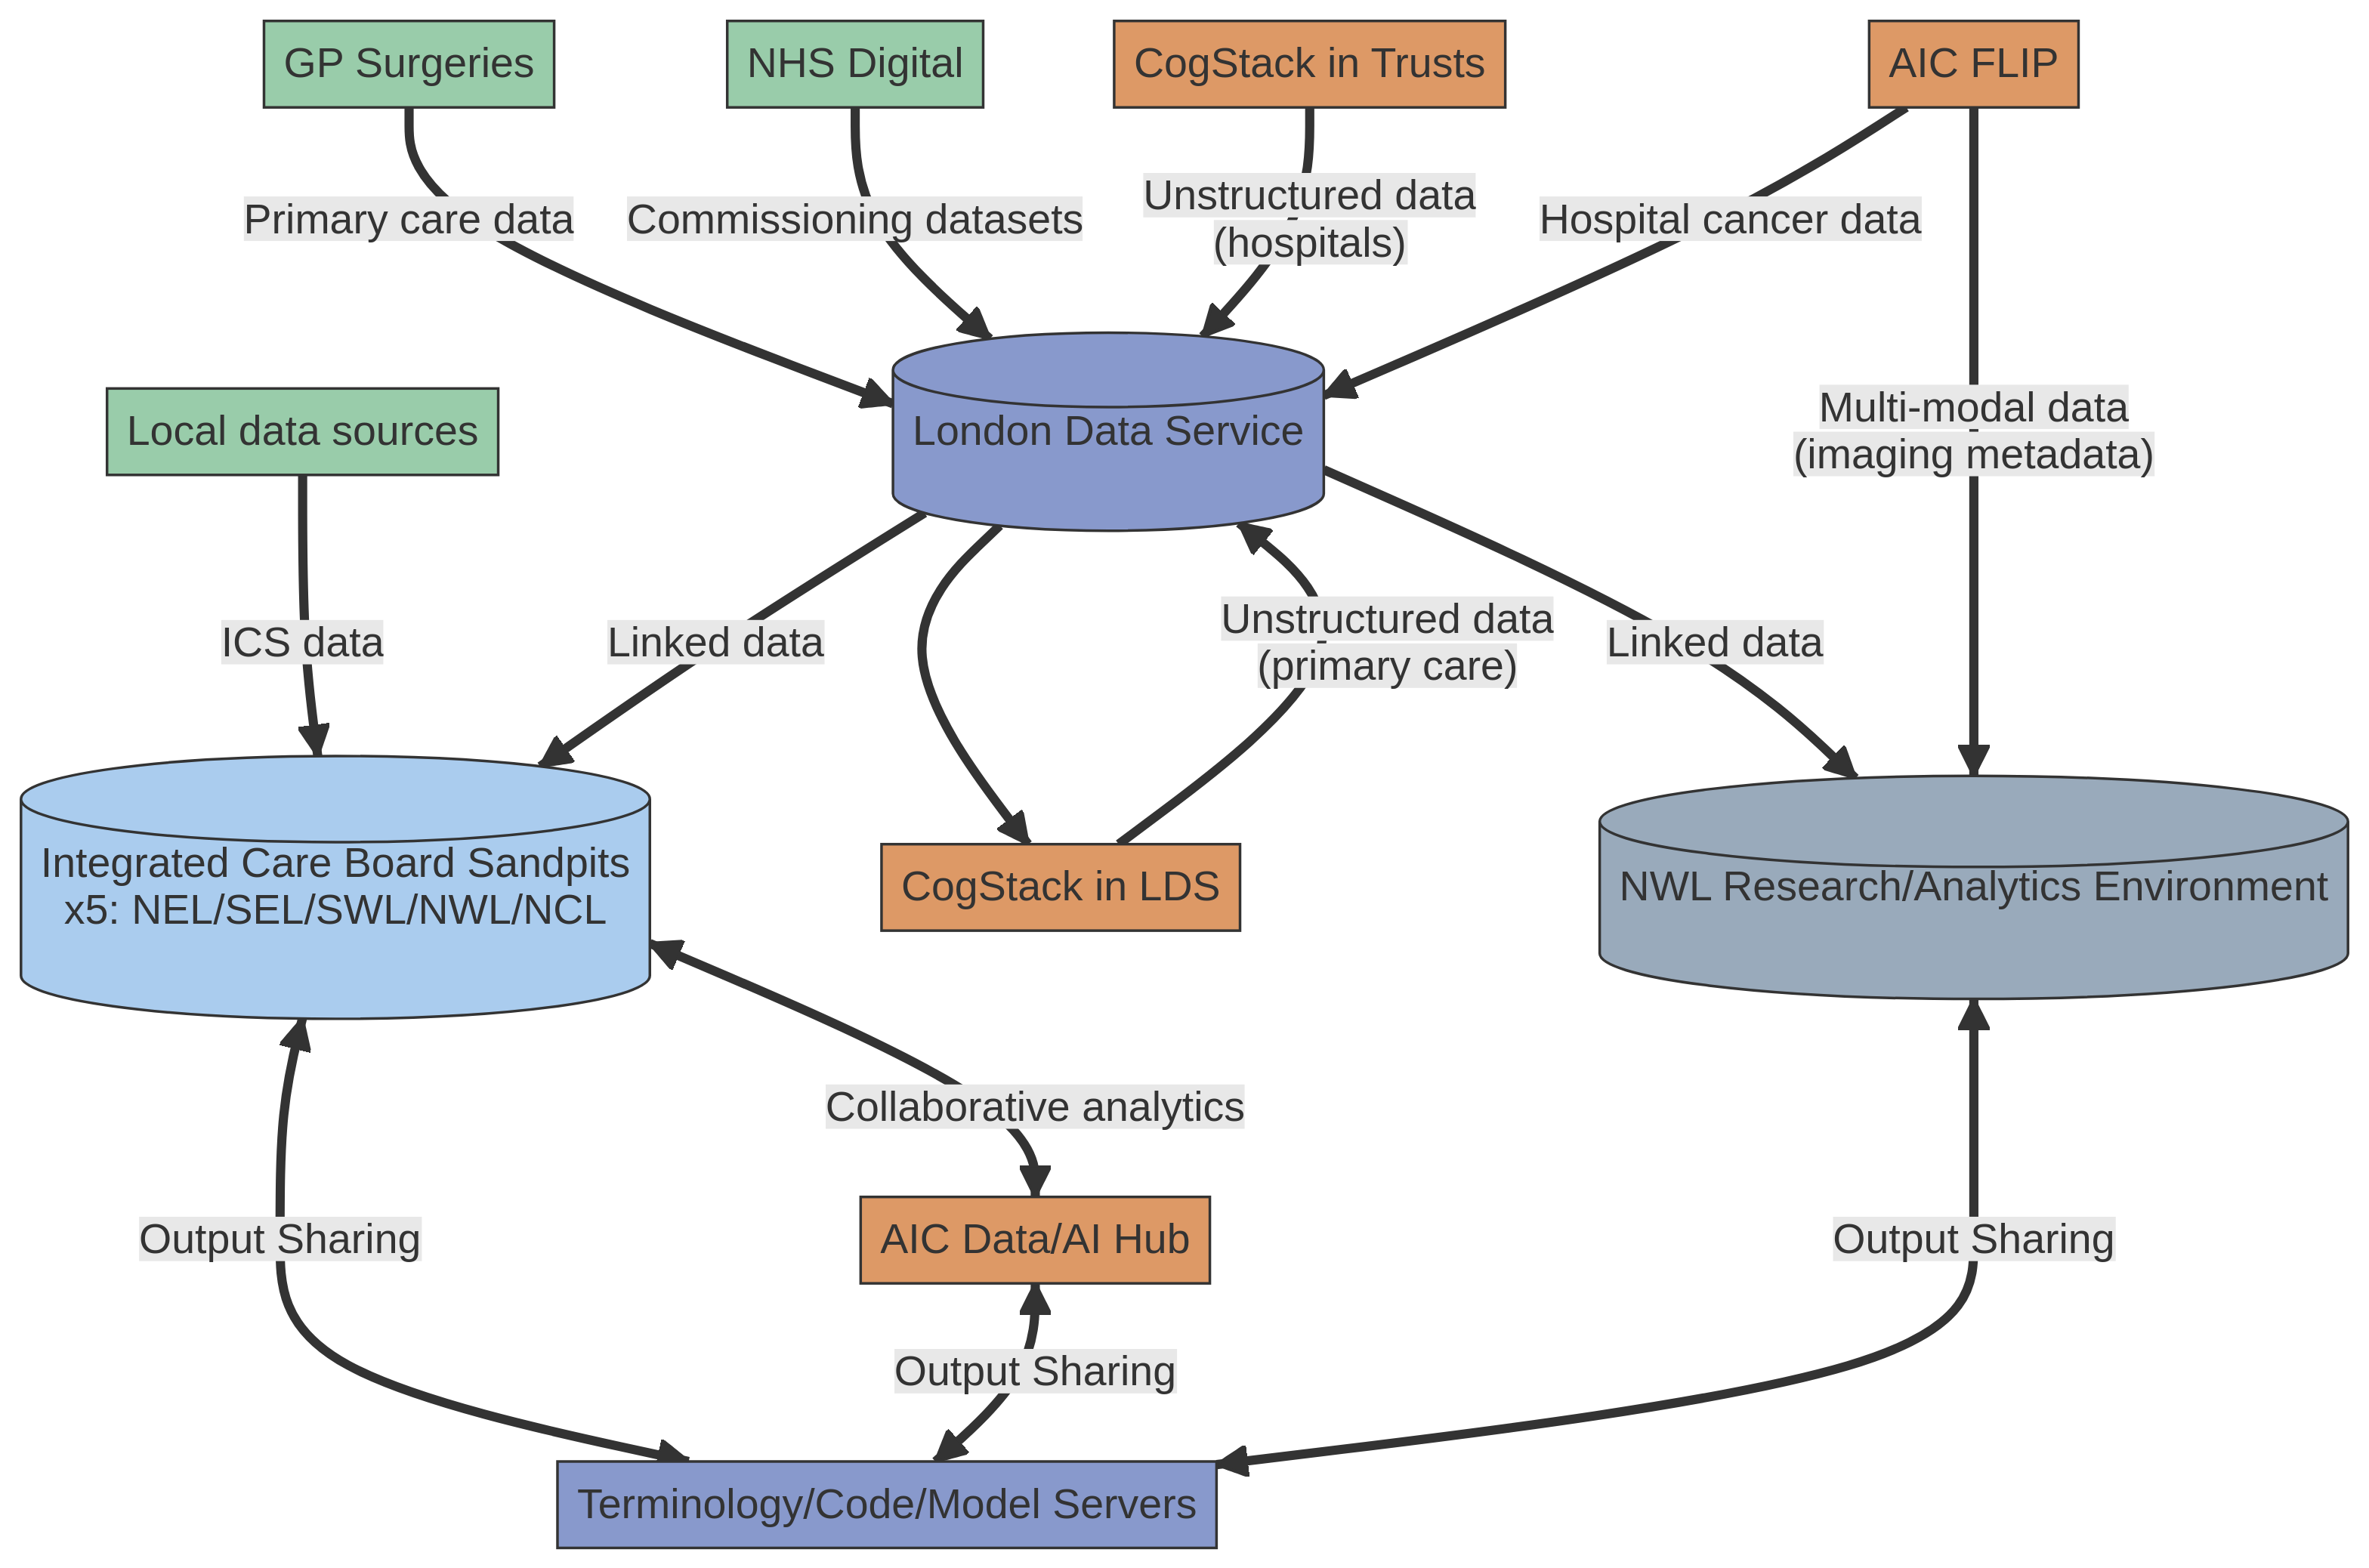
\includegraphics[width=5in,height=3.31in]{index_files/figure-latex/mermaid-figure-3.png}

}

\caption{\label{fig-sde-summary}Summary of SDE components and data
flows. Each London ICB is provisioned with its own data/analytics
environment through the LDS. FLIP = Federated Learning and
Interoperability Platform.}

\end{figure}%

\textsubscript{Source:
\href{https://d3london.github.io/sde_aic_docs/index.qmd.html}{Article
Notebook}}

\subsection{Technology and objectives}\label{technology-and-objectives}

The contribution from the London AIC consists of technology deployment
and supporting expertise, that enable a number of key objectives
(Figure~\ref{fig-aic-objectives}) over the two year programme. This
contribution includes the following:

\begin{enumerate}
\def\labelenumi{(\arabic{enumi})}
\item
  \textbf{Federated Learning and Interoperability Platform (FLIP)}:
  Developed and tested over four years, FLIP consists of (a) secure data
  environments within NHS hospital Trusts for multi-modal imaging data
  and structured data in a common data model; and (b) a mechanism to
  query data and train AI models across these secure enclaves without
  the need to physically transfer data. FLIP is presently installed in
  four major London Trusts. Integrating FLIP into the SDE will enable
  hospital data (such as cancer data) to be surfaced into the LDS, and
  multi-modal capabilities to support research in precision healthcare.
\item
  \textbf{CogStack}: As an advanced natural language processing
  platform, CogStack can turn the large quantities of health information
  that are found in narrative text, into structured and analysable data.
  Currently actively used in Trusts to assist with clinical coding from
  notes and clinic letters, CogStack can surface secondary care and
  cancer pathway data, and previously unseen primary care data, into the
  SDE ecosystem.
\item
  \textbf{AIC Data/AI Hub}: The AIC hosts substantial health data and AI
  implementation expertise, that will provide practical support in data
  operations, engineering, analytics, and machine learning development
  and deployment. A primary aim is to help Integrated Care Boards (ICB)
  migrate data pipelines and analytics onto the LDS, and to produce
  reproducible analytics pipelines for data science and predictive
  analytics capabilities. As the LDS ICB environments share a common
  data model, any pipelines created in collaboration with a single ICB,
  can be adapted and used for any other ICB (or deployed across multiple
  environments to create pan-London insights). This will also facilitate
  shared terminologies, and validating/versioning/serving NHS-owned
  machine learning models across regions.
\end{enumerate}

\begin{figure}

\centering{

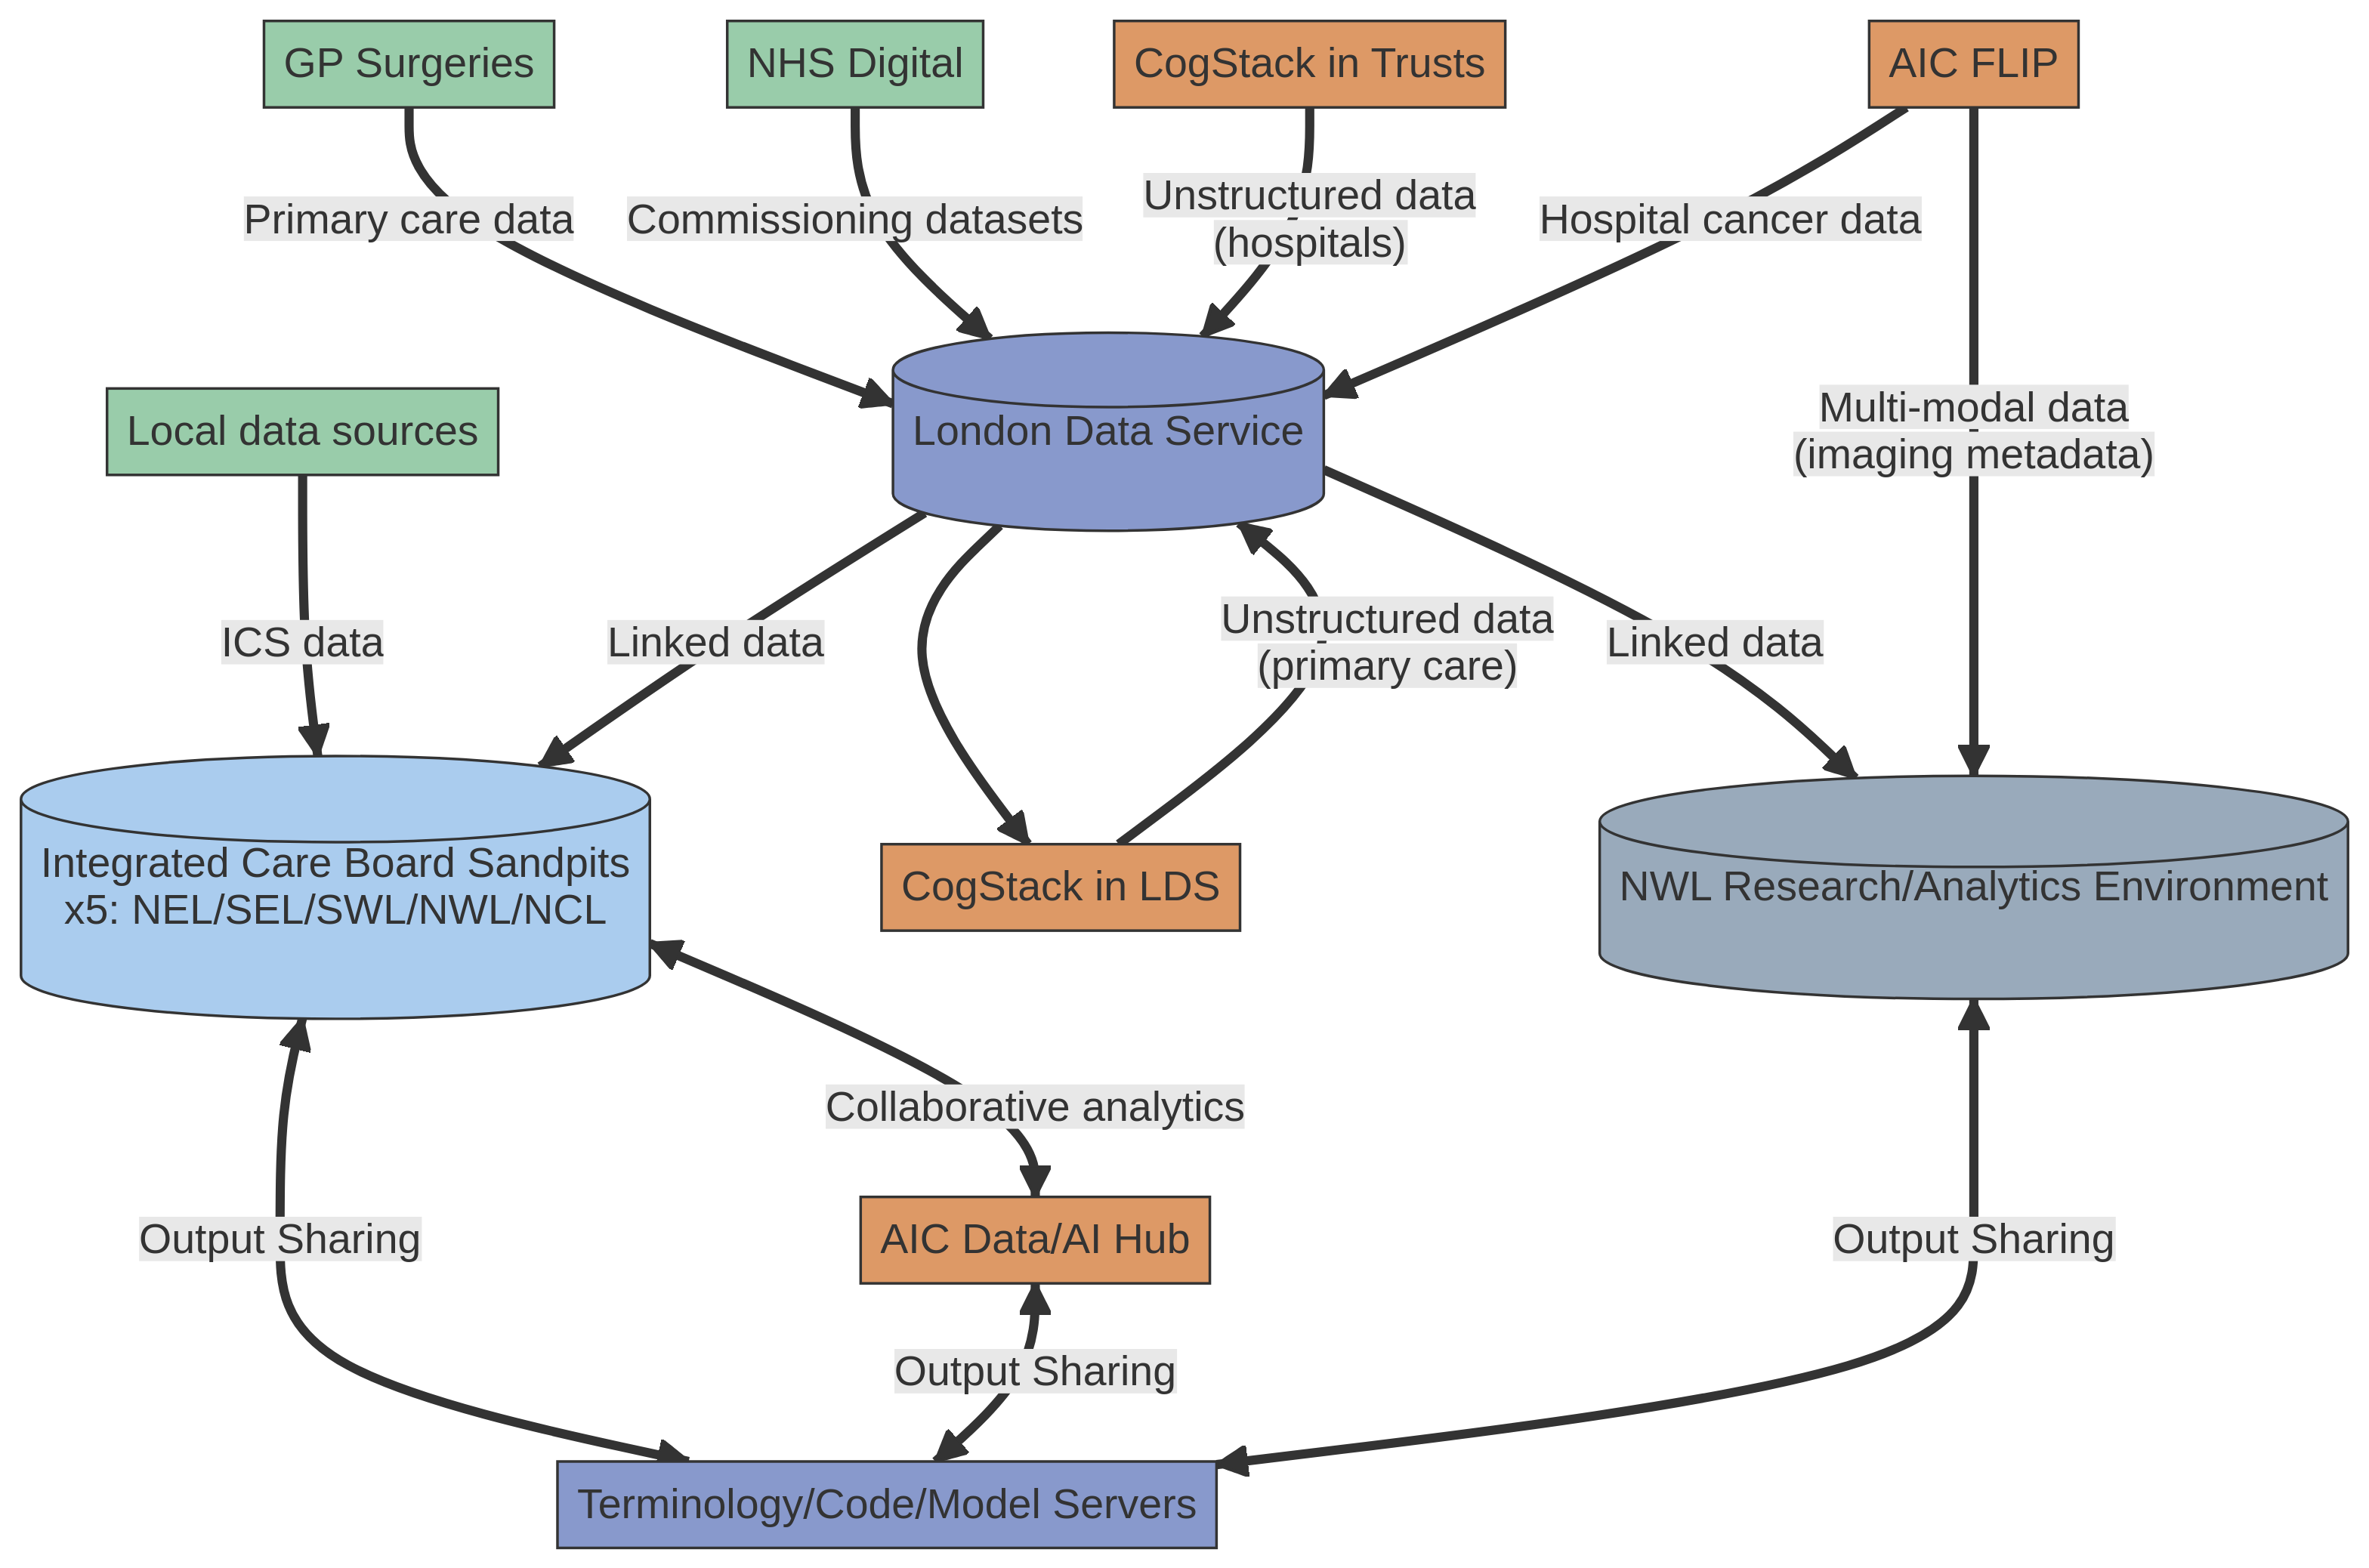
\includegraphics[width=6in,height=2.82in]{index_files/figure-latex/mermaid-figure-4.png}

}

\caption{\label{fig-aic-objectives}Summary of AIC work components and
objectives. FLIP = Federated Learning and Interoperability Platform; ML
= Machine Learning.}

\end{figure}%

\textsubscript{Source:
\href{https://d3london.github.io/sde_aic_docs/index.qmd.html}{Article
Notebook}}

\subsection{Proposed use-cases}\label{proposed-use-cases}

The following use-cases are \emph{examples} of the type of work that are
possible to produce within the SDE ecosystem, conducted collaboratively
between ICB/NHS analytics teams and the AIC. Use-cases align to the
London Health Data Strategy and long term condition priorities, as well
as national programmes such as CORE20PLUS5, and are proposed here
following early discussions with London ICBs. An overarching objective
for any work is to build a reproducible code base that is sharable
between ICBs, and which can be optimised for local uses/dashboards, or
used to create aggregated pan-London insights.

Prior to any of the below projects being conducted, SDE/AIC resources
are also available to help ICBs migrate their current pipelines and
dashboards into the new LDS data environments
(Figure~\ref{fig-aic-objectives}).

\subsubsection{Systematic measurement of group and individual health
inequality}\label{systematic-measurement-of-group-and-individual-health-inequality}

\subsubsection{Cardiovascular disease prevention through decision
intelligence (Hypertension as an
example)}\label{cardiovascular-disease-prevention-through-decision-intelligence-hypertension-as-an-example}

\subsubsection{Actionable admission risk
stratification}\label{actionable-admission-risk-stratification}

\subsubsection{Joining up cancer
pathways}\label{joining-up-cancer-pathways}

\subsubsection{}\label{section}



\end{document}
